\newpage
\section*{1)Написание скриптов. Операторы ветвления}

\subsection*{Написание bash-скрипт, который будет выводить Фамилии И.О. и Вариант группы тремя способами:
\\}

\paragraph{1) Напрямую выводя требуемый текст\\
}

На Рисунке 1.1 изображено окно текстового редактора nano.

Небольшое пояснение к коду:

\#!/bin/bash указывает путь к интерпретатору для исполнения скрипта.С помощью оператора потокового вывода » результат работы скрипта сохраняем в файл \textit{1.data} Результат работы скрипта и вывод содержимого файла \textit{1.data} можно увидеть на Рисунке 1.2.

\vspace{0.5cm}
		\begin{center}
			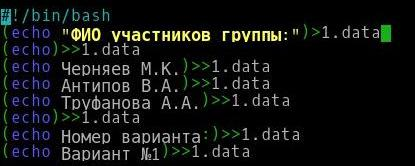
\includegraphics[width=\textwidth]{11.jpg}

			Рисунок 1.1 - Скрипт написанный в nano.\\

			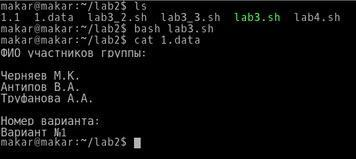
\includegraphics[width=\textwidth]{12.jpg}

			Рисунок 1.2 - Работа скрипта и вывод содержимого файла \textit{1.data}\\

		\end{center}


\paragraph{2) Используя переменную
\\}

На Рисунке 1.3 изображено окно текстового редактора nano. Результат работы скрипта и вывод содержимого файла 2.data можно увидеть на Рисунке 1.4.

\vspace{0.5cm}
		\begin{center}
			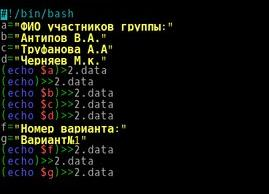
\includegraphics[width=\textwidth]{13.jpg}

			Рисунок 1.3 - Скрипт написанный в nano.\\

			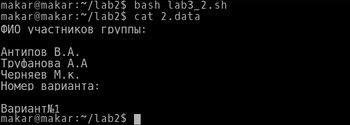
\includegraphics[width=\textwidth]{14.jpg}

			Рисунок 1.4 - Работа скрипта и вывод содержимого файла \textit{2.data}\\

		\end{center}


\paragraph{3) Используя функцию (с локальной переменной)
\\}

На Рисунке 1.5 изображено окно текстового редактора nano. Результат работы скрипта и вывод содержимого файла \textit{3.data} можно увидеть на Рисунке 1.6.

\vspace{0.5cm}
		\begin{center}
			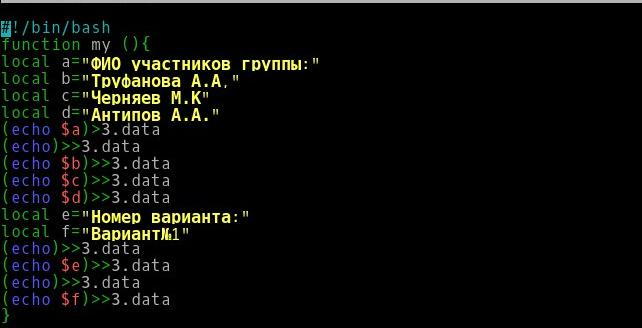
\includegraphics[width=\textwidth]{15.jpg}

			Рисунок 1.5 - Скрипт написанный в nano.\\

			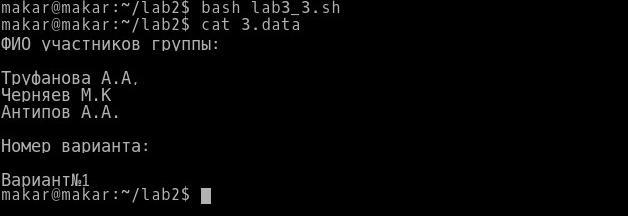
\includegraphics[width=\textwidth]{16.jpg}

			Рисунок 1.6 - Работа скрипта и вывод содержимого файла \textit{3.data}\\

		\end{center}



\subsection*{Анализ (достоинства и недостатки) каждого метода из Задания 2
\\}

Первый метод является самым легким и примитивным, так как для его реализации нужно знать только самые основы написания скриптов на bash. Недостатком является то, что ввод текста каждый раз приходится делать вручную, что не удобно при повторяющемся тексте.

Второй метод является более сложным в применении так как нужно знать основы написания скриптов. Данный метод является более универсальным, так как дублирующийся части текса теперь не нужно вводить снова, можно просто вызвать нужную переменную.

Последний метод самый сложный в реализации, так как для него нужны обширные познания. Этот метод является самым удобным и универсальным, потому что после написания функции, для вывода текста достаточно вызвать такое количество раз, сколько раз нужно вывести данный текст.\\



\subsection*{Написание скрипта, который будет запрашивать ввести число (учесть возможность ввода не числового значения как ошибки с оповещением и повторным запросом).
\\}

Небольшое пояснение к коду:

Для реализации повторного запроса задаем данный алгоритм ветвления в функции, и при необходимости повторного запроса создаем рекурсию-вызов функцией саму себя, пока не будет достигнут удовлетворяющий нас вариант. На Рисунке 1.7 изображено окно текстового редактора nano. Результат работы скрипта и вывод содержимого файла 4.data можно увидеть на Рисунке 1.8.

\vspace{0.5cm}
		\begin{center}
			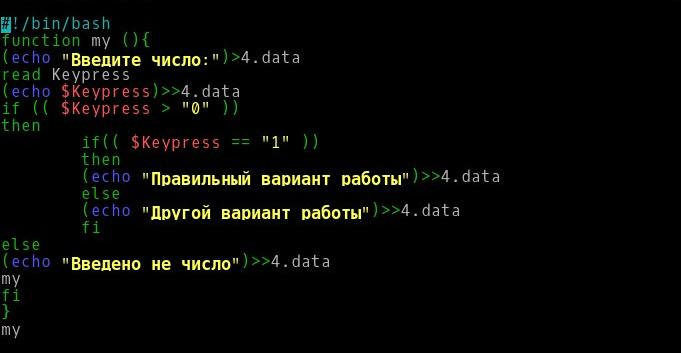
\includegraphics[width=\textwidth]{17.jpg}

			Рисунок 1.7 - Скрипт написанный в nano.\\

			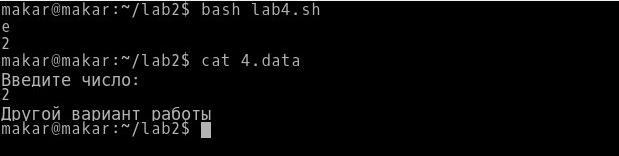
\includegraphics[width=\textwidth]{18.jpg}

			Рисунок 1.8 - Работа скрипта и вывод содержимого файла \textit{3.data}\\

		\end{center}